\subsection{Ultrafast NMR}
\label{subsec:poise__epsi}

The final example of a single-parameter POISE optimisation is also the most complicated: it pertains to the EPSI acquisition technique, which was previously introduced in \cref{sec:pureshift__epsidosy}.
EPSI acquisition allows signals from different slices of the sample to be simultaneously detected in a single FID, and (in liquid-state NMR) has most famously been used in the context of \textit{ultrafast} 2D experiments\autocite{Frydman2002PNASUSA,Pelupessy2003JACS,Frydman2003JACS,Tal2010PNMRS,Giraudeau2014ARAC,Gouilleux2018ARNMRS}, where the $t_1$ evolution is spatially encoded and read out using the EPSI technique.

\begin{figure}[htb]
    \centering
    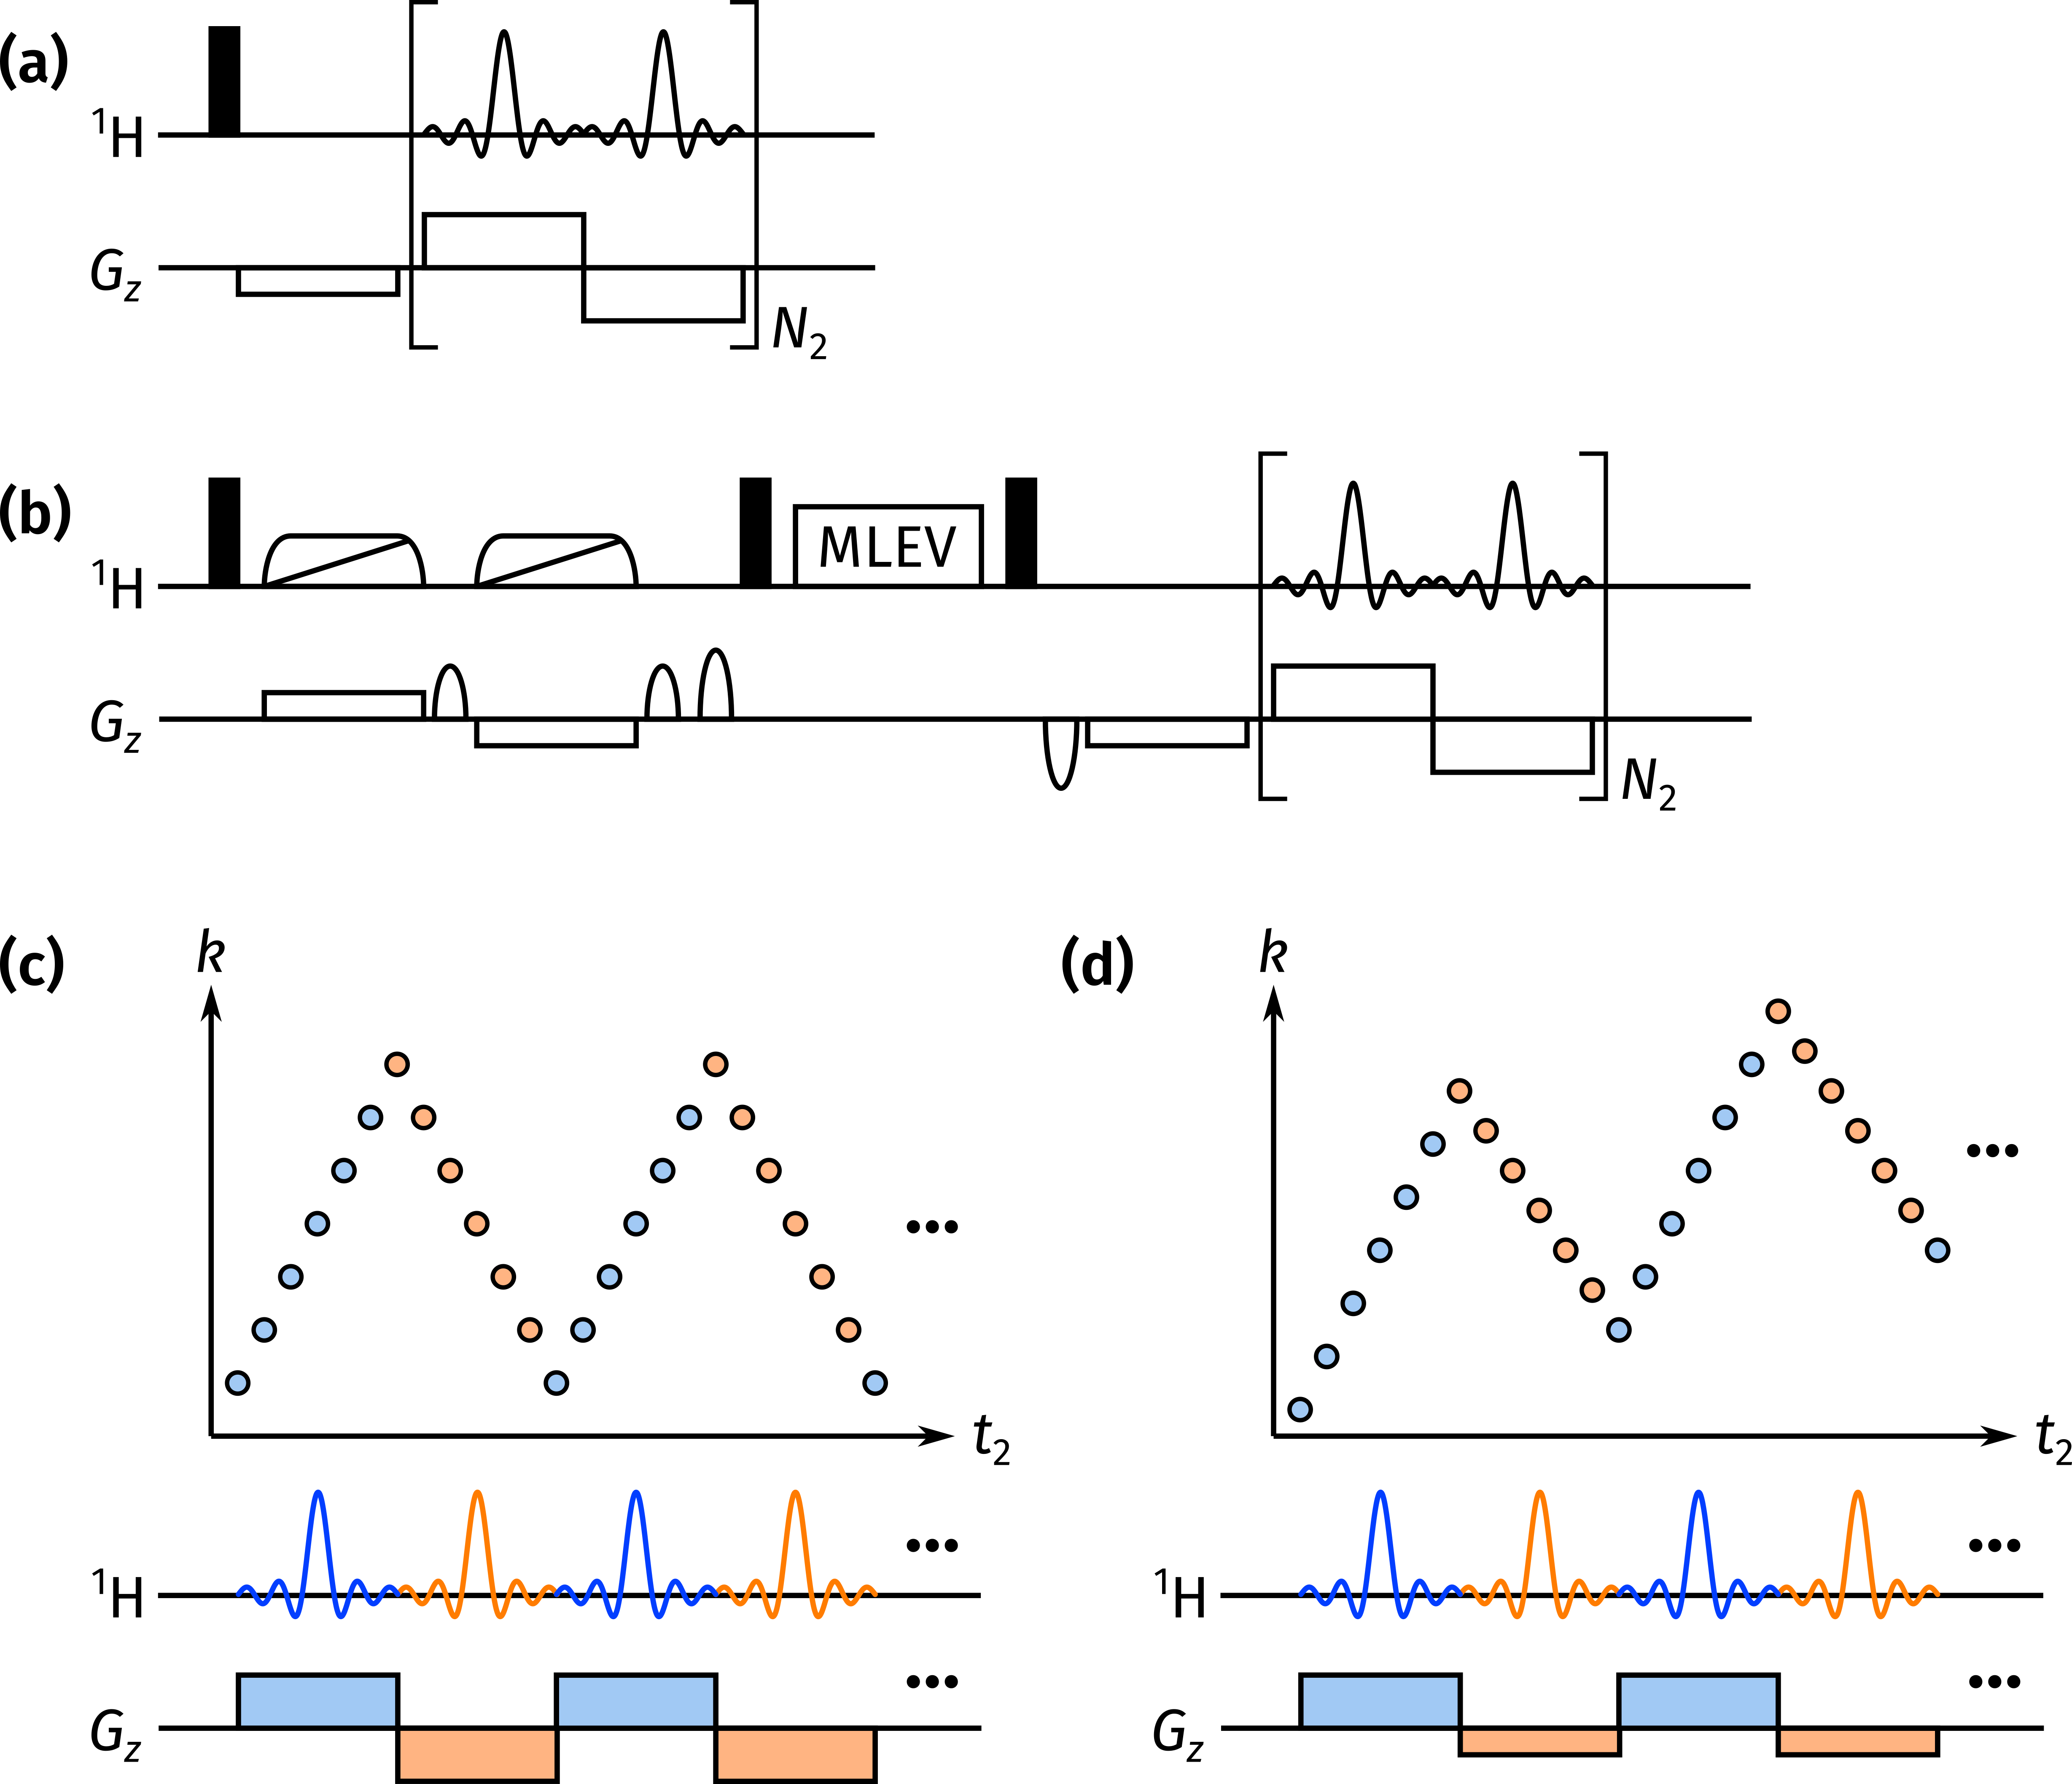
\includegraphics[draft=false]{pp/poise/epsi.png}
    {\phantomsubcaption\label{fig:poise_epsi_zgepsi}}
    {\phantomsubcaption\label{fig:poise_epsi_tocsyepsi}}
    {\phantomsubcaption\label{fig:poise_epsi_epsicorrect}}
    {\phantomsubcaption\label{fig:poise_epsi_epsiwrong}}
    \caption[Pulse sequences used for EPSI optimisation]{
        Pulse sequences used for EPSI optimisation, and depiction of the $(k, t_2)$ data matrices thus obtained.
        \textbf{(\subref{fig:poise_epsi_zgepsi})} Pulse--EPSI experiment.
        \textbf{(\subref{fig:poise_epsi_tocsyepsi})} Ultrafast TOCSY experiment; gradients were set up according to the protocol of Giraudeau et al.\autocite{Gouilleux2018ARNMRS}
        \textbf{(\subref{fig:poise_epsi_epsicorrect})} Illustration of the $(k, t_2)$ data matrix obtained during an EPSI acquisition period.
        Blue dots indicate data acquired during a positive gradient, and orange dots data acquired during the negative gradient.
        \textbf{(\subref{fig:poise_epsi_epsiwrong})} The $(k, t_2)$ data matrix obtained when the positive and negative EPSI gradients (blue and orange in the pulse sequences) are not balanced.
        In this case, the negative gradient is slightly weaker, leading to a `drift' towards larger values of $k$.
    }
    \label{fig:poise_epsi}
\end{figure}

During an EPSI acquisition period, alternating gradients of equal magnitude but opposite sign are applied, as shown in \cref{fig:poise_epsi_zgepsi,fig:poise_epsi_tocsyepsi}. Each data point collected therefore depends not only on $t_2$ (the acquisition time domain) but also on $k$, a wavenumber which measures the extent of gradient dephasing caused by the acquisition gradients:
\begin{equation}
    \label{eq:epsi_k_space}
    k = \int_0^{t_2} \gamma G(t) \,\mathrm{d}t.
\end{equation}
This value of $k$ increases during positive gradients and decreases during negative gradients, leading to a zigzag pattern in $k$-space, all while $t_2$ is still increasing (\cref{fig:poise_epsi_epsicorrect}).
The \textit{prephasing gradient} immediately before acquisition has the same duration as the EPSI gradients, but has half the amplitude, meaning that $k$ begins from a negative value, specifically, $k_\text{max} / 2$, where $k_\text{max}$ is the change in $k$ caused by one complete positive EPSI gradient.
As explained in previous reviews\autocite{Frydman2003JACS}, the spatial profile $f(z)$ can be obtained by Fourier transformation of the $k$ domain.
Alternatively, since $t_1$ is proportional to $z$ and the indirect-dimension frequency $F_1$ is itself obtained through Fourier transformation of the $t_1$-domain, the $F_1$ and $k$ domains are in fact directly proportional: no Fourier transform is required along this axis to obtain the indirect-dimension frequencies.

This rapid alternating of gradients is very demanding on spectrometers, and it is often the case that the positive and negative EPSI gradients---although \textit{nominally} specified with the same amplitude---are not perfectly balanced.
This causes a `drift' in the $k$-domain over time, as illustrated in \cref{fig:poise_epsi_epsiwrong}.
In this section, POISE is used to perform an \textit{instrument-specific} optimisation in order to correct for this effect.


\subsubsection{Optimisation setup}

To measure the drift in $k$-space, it is easiest to use a pulse sequence for which there is no spatial encoding; the pulse--EPSI experiment (\cref{fig:poise_epsi_zgepsi}) is perfectly suited for this.
In the pulse programme, I multiplied the amplitudes of the negative gradients by a factor $\alpha$, represented as \texttt{CNST16} in TopSpin:
the objective of POISE is therefore to determine the optimum value for this which minimises the drift.
Calculating this drift requires fairly substantial processing, which is most easily done inside the cost function using \texttt{numpy} functions (rather than, for example, a TopSpin AU script).
The \texttt{epsi\_gradient\_drift} cost function therefore consists of the following steps:
\begin{enumerate}
    \item reading in the 1D FID and reshaping it into a 2D $(k, t_2)$ matrix;
    \item discarding data obtained during negative gradients;
    \item determining, for each point in $t_2$, the value of $k$ for which the maximum signal is found;
    \item performing linear regression on these points and obtaining the slope of $k$ against $t_2$, the absolute value of which directly represents the extent of $k$-space drifting.
\end{enumerate}

\begin{figure}[htb]
    \centering
    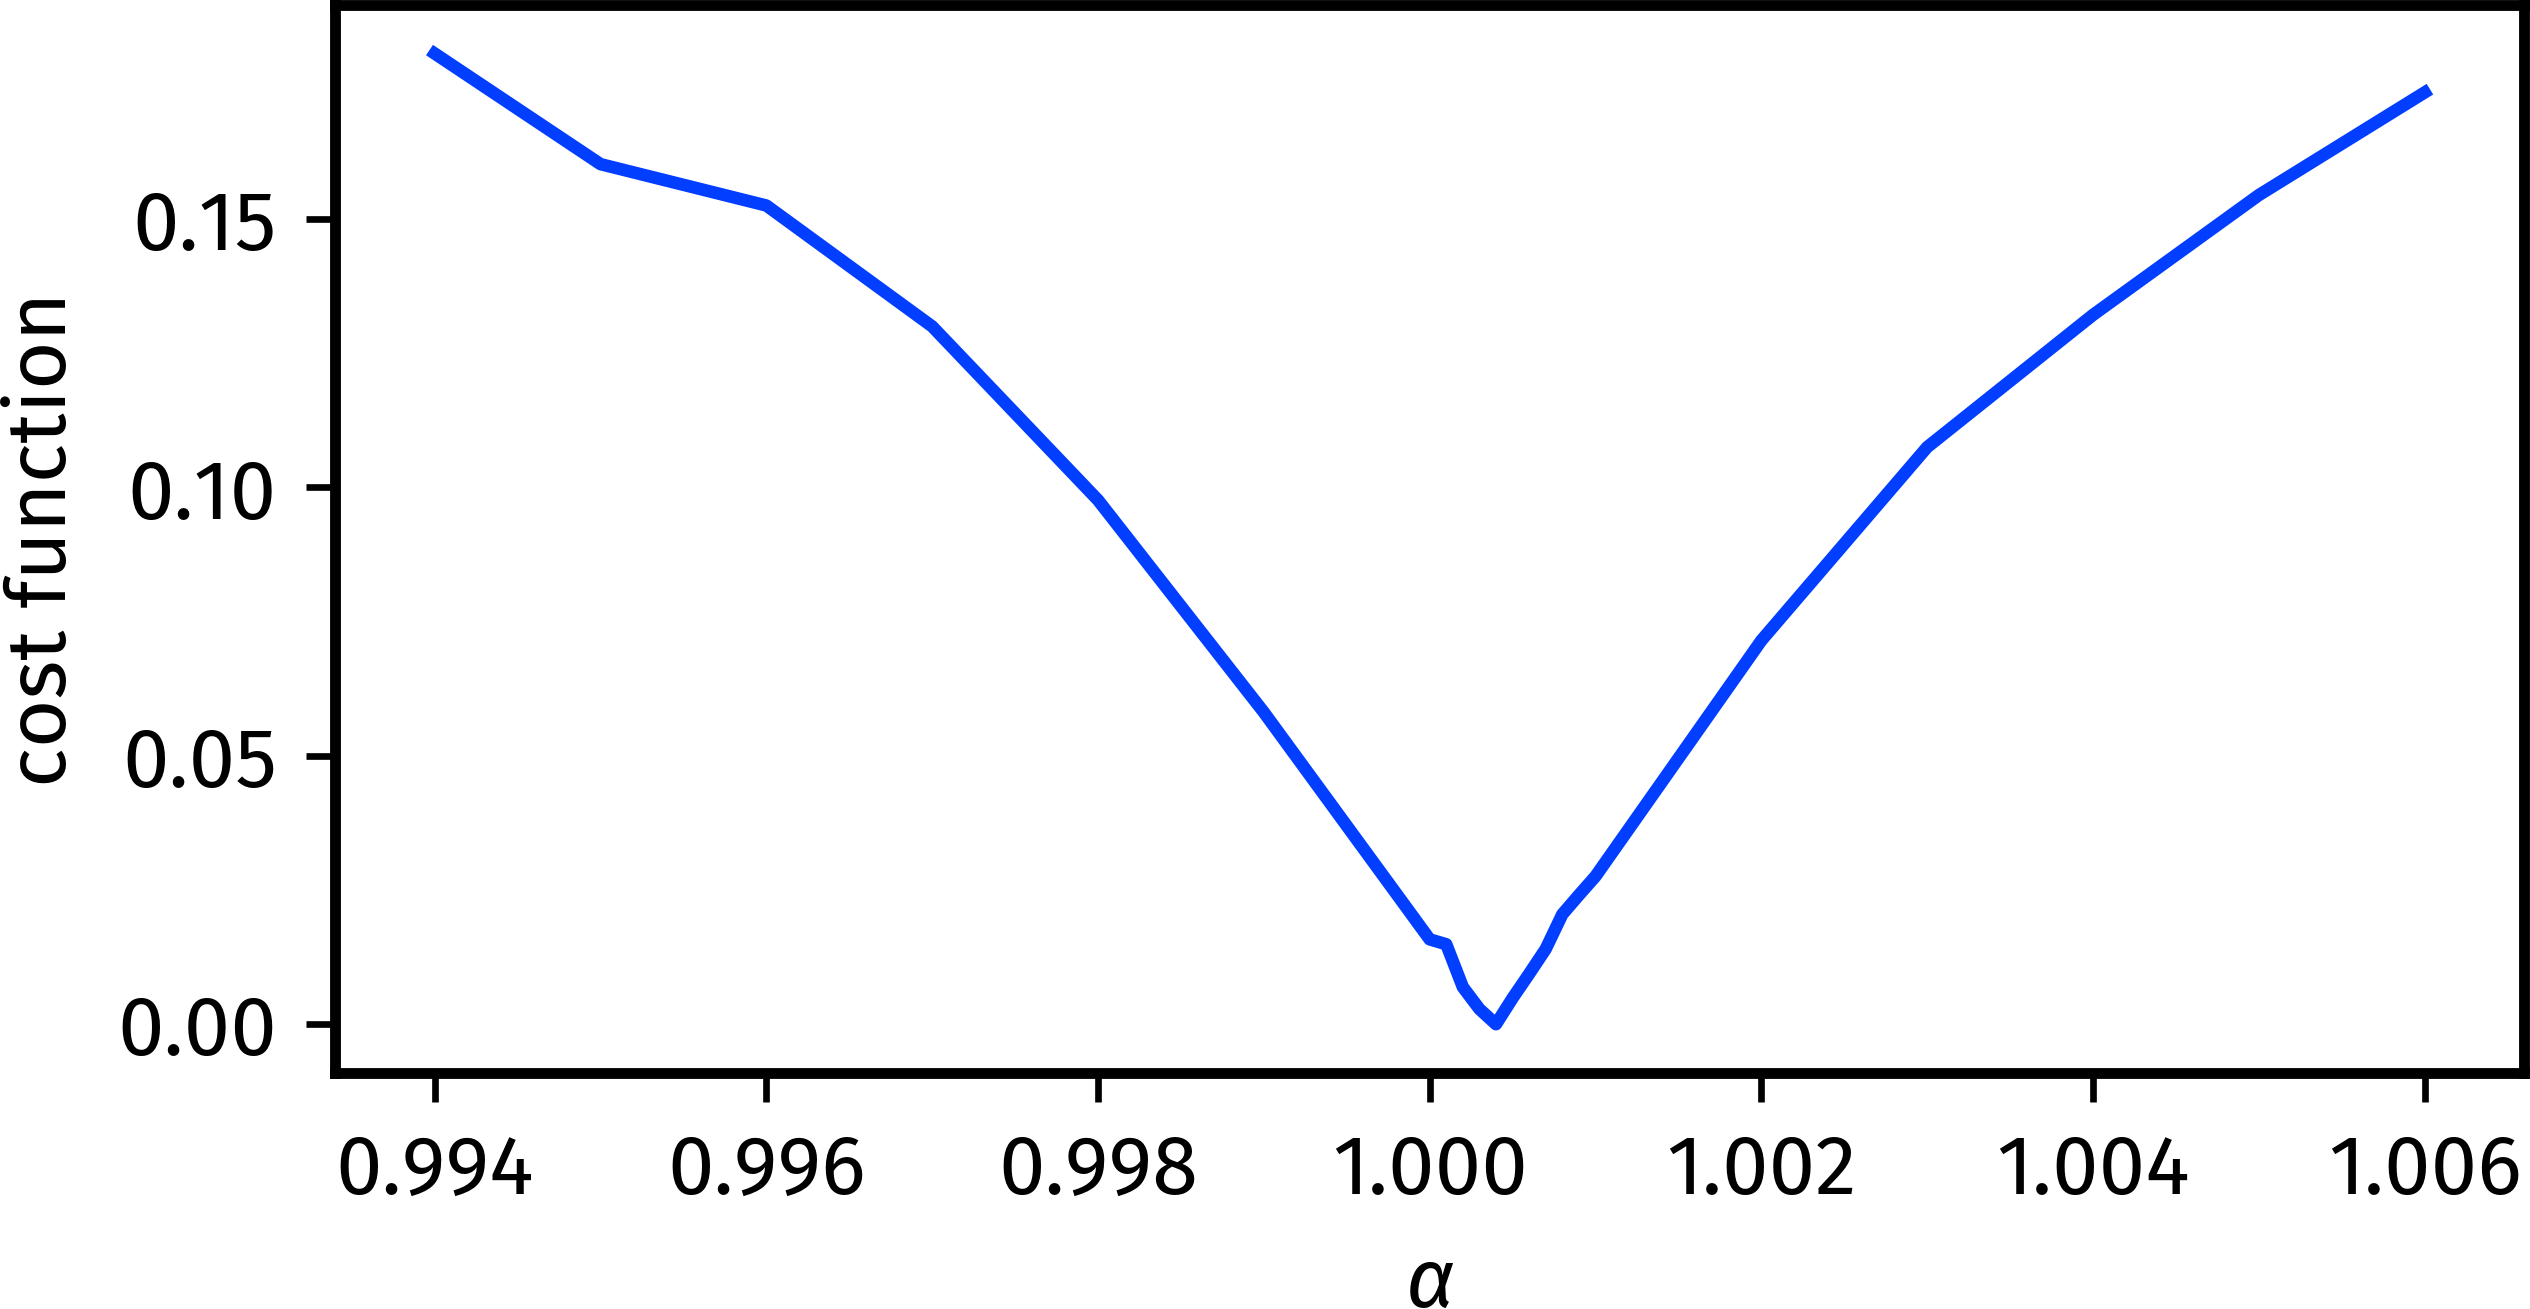
\includegraphics[]{figures/poise/epsi_scan.png}
    \caption[Reference grid search for EPSI optimisation]{
        Reference grid search for EPSI optimisation.
        \datacode{6F-210316}
    }
    \label{fig:poise_epsi_scan}
\end{figure}

Since the cost function constructed here was relatively complicated, I carried out a reference grid search to confirm that it was working as intended (\cref{fig:poise_epsi_scan}).
This yielded an expected optimum of $\alpha = 1.0004$.
(The sample used here was ferulic acid, but in principle this should not matter as the drift is due to the spectrometer and not the sample.)

To save time in the optimisation itself, I reused the strategy of setting \texttt{DS=0} and \texttt{NS=1}.
As before, since each FE is separated by approximately five seconds of processing and spectrometer initialisation, this means that there is no need for another recovery delay; thus, \texttt{D1} was set to \SI{0.5}{\s}.
However, note that such a short recovery delay should \textit{not} be used if \texttt{DS} is larger than 0 or \texttt{NS} larger than 1: EPSI acquisitions should not be carried out in rapid succession.
Furthermore, \texttt{AQ} should be kept under \SI{100}{\ms}.


\subsubsection{Optimisation results}

\begin{table}[htb]
    \hbadness=10000
    \centering
    \begin{tabular}{ccccc}
        \toprule
        Entry & Algorithm & Optimum found      & FEs & Time taken (\si{\s}) \\
        \midrule
        1     & NM        & 1.000375           & 10  & 49--52               \\
        2     & MDS       & 1.000375           & 10  & 49--50               \\
        3     & BOBYQA    & 1.000383--1.000388 & 7   & 34--35               \\
        \bottomrule
    \end{tabular}
    \caption{
        Results of EPSI gradient imbalance optimisations.
        Note that in practice, all of these optimisations actually converge to $\alpha = 1.0004$; the extra decimal place is not used by the spectrometer (see text for further discussion).
        The POISE routine used here is: \mintinline[breaklines]{json}{{"name": "epsi", "pars": ["cnst16"], "lb": [0.99], "ub": [1.01], "init": [1.0], "tol": [0.0001], "cf": "epsi_gradient_drift", "au": "poise_1d"}}.
        \datacode{6F-210316}
    }
    \label{tbl:poise_epsi}
\end{table}

In the event, all three optimisation algorithms successfully find the the optimal value of $\alpha$ in under a minute (\cref{tbl:poise_epsi}).
It is worth clarifying one subtlety of POISE here.
In the table, the optima are quoted to a rather greater precision than one might expect at first: however, the actual precision of the optimisation result is not given by the number of significant figures,\footnote{The entire concept of `significant figures' is a very crude way of expressing uncertainty anyway.} but rather a combination of two factors:

\begin{itemize}
    \item first, the \textit{optimisation tolerance}, which is purely determined by the optimisation routine. Thus, in \cref{tbl:poise_epsi}, the optimum of 1.000375 actually means $1.000375 \pm 0.0001$ (and not $1.000375 \pm 0.0000005$, as `significant figures' would imply); and
    \item second, the available \textit{spectrometer resolution}, which represents how precisely the spectrometer can implement a given parameter value.
        In this case, the available resolution is $0.0001$, which means that even if we input the `optimum' of $\alpha = 1.000375$, the experiment is executed with $\alpha = 1.0004$ (see also \cref{fig:epsi_spec}).
        The optimisation algorithm has no knowledge of this, so it still reports a value of $1.000375$.
        When reporting optima from POISE, users should be wary of this.
\end{itemize}

This further underlines the importance of choosing a sensible optimisation tolerance: it should be \textit{at least} as large as the instrument resolution (larger values can be used when an extremely accurate result is not needed).

\begin{figure}[htb]
    \centering
    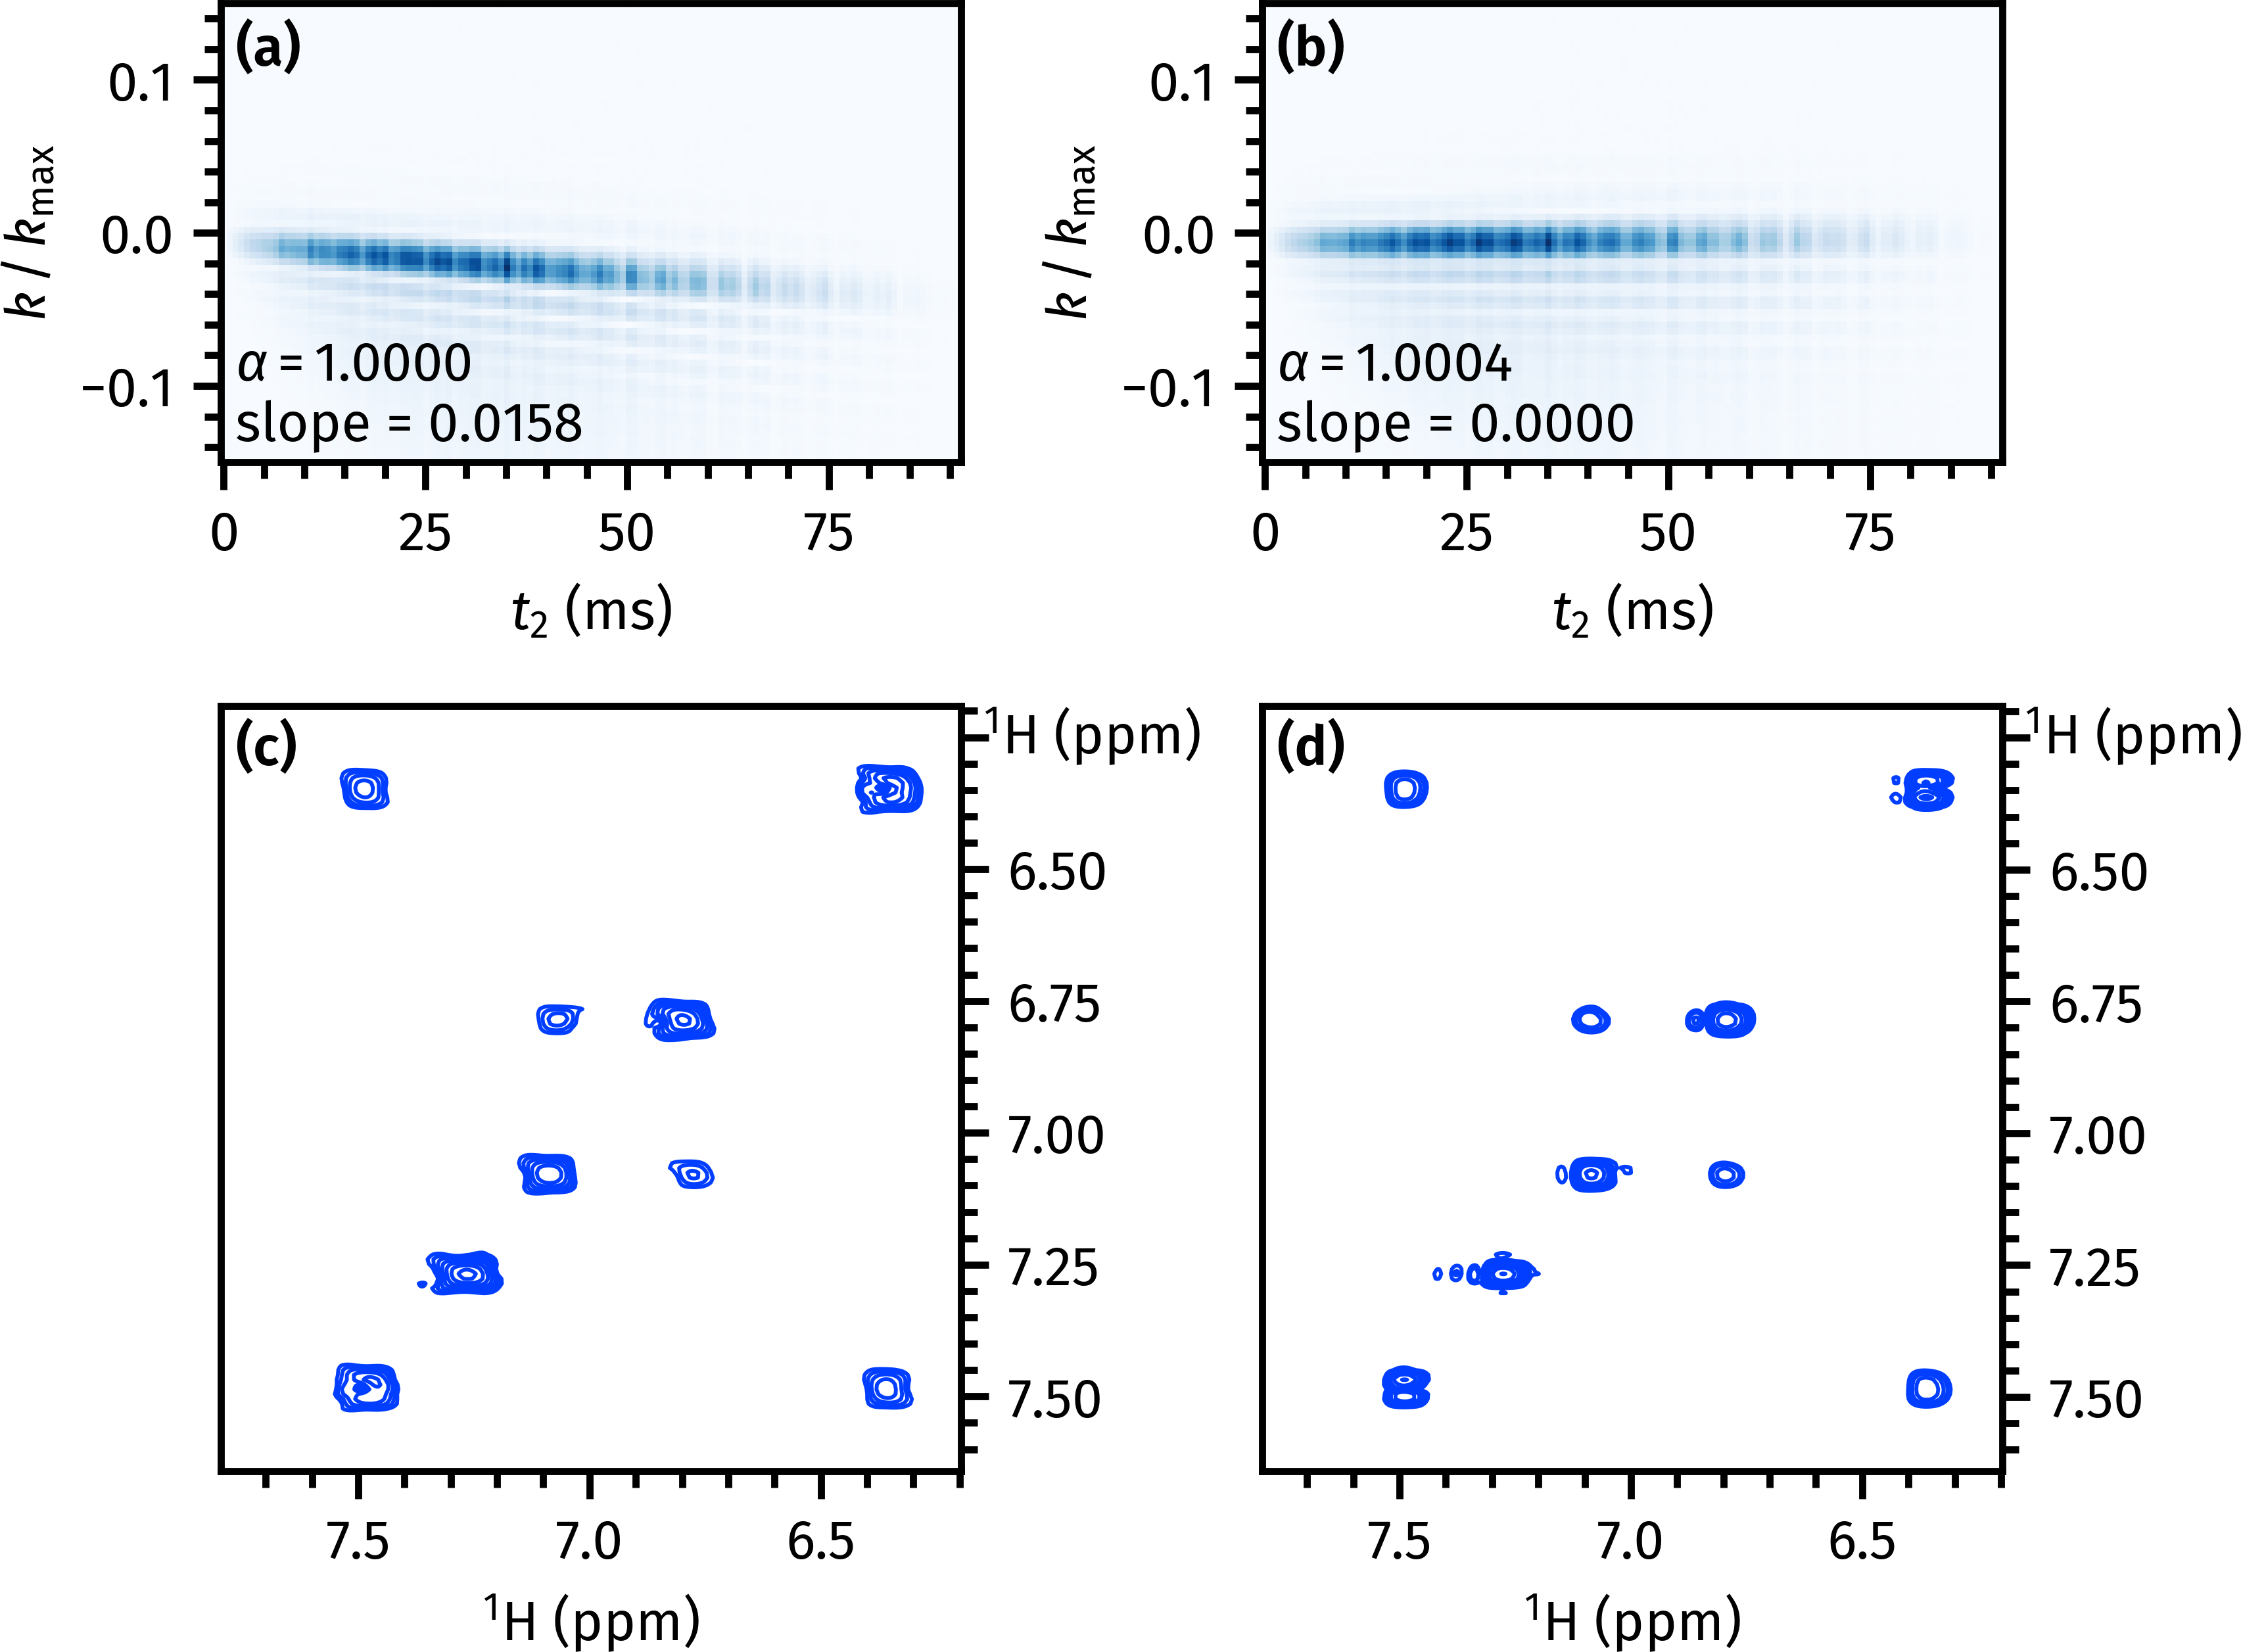
\includegraphics[draft=false]{poise/epsi_spec.png}
    {\phantomsubcaption\label{fig:epsi_spec_kt_noopt}}
    {\phantomsubcaption\label{fig:epsi_spec_kt_opt}}
    {\phantomsubcaption\label{fig:epsi_spec_tocsy_noopt}}
    {\phantomsubcaption\label{fig:epsi_spec_tocsy_opt}}
    \caption[Comparison between unoptimised and optimised EPSI spectra]{
        \textbf{(\subref{fig:epsi_spec_kt_noopt},\subref{fig:epsi_spec_kt_opt})} Magnitude-mode $(k, t_2)$ data matrices obtained from the pulse--EPSI experiment, before and after optimisation of $\alpha$ respectively.
        \textbf{(\subref{fig:epsi_spec_tocsy_noopt},\subref{fig:epsi_spec_tocsy_opt})} The corresponding 2D ultrafast TOCSY spectra, recorded with the unoptimised and optimised value of $\alpha$ respectively.
        The MLEV mixing period used was \SI{10}{\ms}.
    }
    \label{fig:epsi_spec}
\end{figure}

The $(k, t_2)$ data matrices obtained from the excitation--EPSI pulse sequence are shown in \cref{fig:epsi_spec_kt_noopt,fig:epsi_spec_kt_opt}.
In the former, where the default value of $\alpha = 1$ is used, there is a noticeable drift in $k$-space.
This is removed in the optimised experiment with $\alpha = 1.0004$.
Using the optimised value of $\alpha$ in fact leads to much improved ultrafast spectra, such as the TOCSY spectra recorded with the pulse sequence in \cref{fig:poise_epsi_tocsyepsi}.
\Cref{fig:epsi_spec_tocsy_noopt,fig:epsi_spec_tocsy_opt} show respectively the ultrafast TOCSY spectra recorded without and with optimisation of the gradient ratio $\alpha$.
In the latter, substantial improvements in lineshapes are obtained, even allowing some couplings to be properly resolved in the indirect dimension.
In principle, this $k$-drift could be compensated for by shearing of the $(k, t_2)$ data matrix prior to Fourier transformation.
However, similar improvements in lineshapes could not be accomplished using the \texttt{ufproc.py} processing script provided by Giraudeau et al.\autocite{Gouilleux2018ARNMRS} (and I did not attempt to do so manually).
